% System Threat Forecaster Presentation
\documentclass[aspectratio=169]{beamer}

% Theme
\usetheme{Madrid}
\usecolortheme{default}

% Packages
\usepackage{graphicx}
\usepackage{booktabs}
\usepackage{amsmath}
\usepackage{hyperref}
\usepackage{tikz}
\usetikzlibrary{shapes,arrows,positioning}

% Title Information
\title{System Threat Forecaster}
\subtitle{AICTE QIP PG Certification Programme on\\``Deep Learning: Fundamentals and Applications''}
\author{Milav Jayeshkumar Dabgar}
\institute{%
    Department of Electronics Engineering\\
    Sardar Vallabhbhai National Institute of Technology, Surat
}
\date{December 2025}

\begin{document}

% Title Slide
\begin{frame}
\titlepage
\end{frame}

% Outline
\begin{frame}{Outline}
\begin{columns}[t]
\column{0.5\textwidth}
\tableofcontents[sections={1-3}]

\column{0.5\textwidth}
\tableofcontents[sections={4-7}]
\end{columns}
\end{frame}

% Section 1: Introduction
\section{Introduction}

\subsection{Background}
\begin{frame}{Background}
\begin{itemize}
    \item Cybersecurity threats are increasingly sophisticated
    \item Malware poses significant risks:
    \begin{itemize}
        \item Data breaches and financial losses
        \item System compromise and data theft
        \item Operational disruptions
    \end{itemize}
    \item Traditional signature-based antivirus solutions struggle with:
    \begin{itemize}
        \item Zero-day attacks and polymorphic malware
        \item Evolving threat landscapes
    \end{itemize}
    \item \textbf{Machine Learning} offers proactive, behavior-based threat detection
\end{itemize}
\end{frame}

\subsection{Problem Statement}
\begin{frame}{Problem Statement}
\begin{block}{Primary Challenge}
Predict malware infections based on system properties using 100,000 samples with 76 diverse features
\end{block}

\vspace{0.3cm}

\textbf{Specific Challenges:}
\begin{itemize}
    \item High dimensionality: 48 numerical + 28 categorical features
    \item Missing values in critical features (RealTimeProtectionState, CityID)
    \item Balanced but complex dataset (50.52\% positive, 49.48\% negative)
    \item Need for efficient and accurate classification
\end{itemize}
\end{frame}

% Section 2: Data Analysis
\section{Data Analysis}

\subsection{Dataset Overview}
\begin{frame}{Dataset Overview}
\begin{center}
\includegraphics[width=0.75\textwidth,height=0.7\textheight,keepaspectratio]{figures/dataset_overview.png}
\end{center}
\end{frame}

\begin{frame}{Dataset Characteristics}
\begin{columns}[T]
\column{0.5\textwidth}
\includegraphics[width=\textwidth]{figures/target_distribution.png}

\column{0.5\textwidth}
\includegraphics[width=\textwidth]{figures/feature_types.png}
\end{columns}
\end{frame}

\subsection{Data Quality}
\begin{frame}{Data Quality Overview}
\begin{center}
\includegraphics[width=0.85\textwidth,height=0.75\textheight,keepaspectratio]{figures/data_quality_overview.png}
\end{center}
\end{frame}

\begin{frame}{Missing Values Analysis}
\begin{center}
\includegraphics[width=0.85\textwidth]{figures/missing_values.png}
\end{center}
\end{frame}

\subsection{Feature Analysis}
\begin{frame}{Key Features Analysis}
\begin{columns}[T]
\column{0.5\textwidth}
\textbf{Most Predictive Features:}
\begin{enumerate}
    \item \textbf{AntivirusConfigID} \\ Correlation: 0.118
    \item \textbf{TotalPhysicalRAMMB} \\ Correlation: 0.066
    \item \textbf{IsSystemProtected} \\ Correlation: 0.062
    \item \textbf{IsGamer} \\ Correlation: 0.061
\end{enumerate}

\vspace{0.3cm}
\begin{alertblock}{Key Insight}
Security configuration has the highest predictive power
\end{alertblock}

\column{0.5\textwidth}
\includegraphics[width=\textwidth]{figures/feature_correlation.png}
\end{columns}
\end{frame}

\begin{frame}{Feature Correlation Analysis}
\begin{center}
\includegraphics[width=0.85\textwidth,height=0.75\textheight,keepaspectratio]{figures/feature_importance_detailed.png}
\end{center}
\end{frame}

\begin{frame}{Feature Correlation Heatmap}
\begin{center}
\includegraphics[width=0.75\textwidth,height=0.7\textheight,keepaspectratio]{figures/correlation_heatmap.png}
\end{center}
\end{frame}

% Section 3: Objectives
\section{Objectives}

\subsection{Project Goals}
\begin{frame}{Project Objectives}
\begin{enumerate}
    \item \textbf{Data Preprocessing}: Implement comprehensive preprocessing techniques
    \begin{itemize}
        \item Missing value imputation
        \item Feature encoding and normalization
    \end{itemize}
    
    \item \textbf{Feature Engineering}: Develop strategies to enhance model performance
    
    \item \textbf{Model Development}: Train and evaluate multiple ML models
    
    \item \textbf{Performance Optimization}: Hyperparameter tuning and model selection
    
    \item \textbf{Model Comparison}: Systematic evaluation using standard metrics
    
    \item \textbf{Deployment Ready}: Create maintainable, production-ready codebase
\end{enumerate}
\end{frame}

% Section 4: Methodology
\section{Methodology}

\subsection{Data Processing Pipeline}
\begin{frame}{Data Processing Pipeline}
\begin{center}
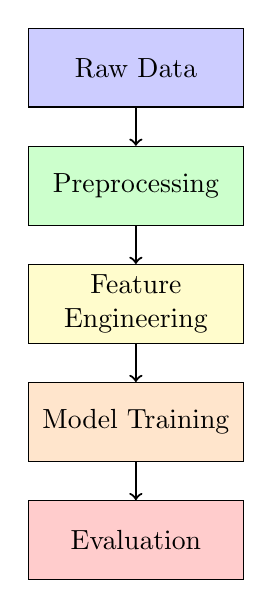
\begin{tikzpicture}[node distance=1.5cm, auto]
    \node (data) [rectangle, draw, fill=blue!20, text width=2.5cm, text centered, minimum height=1cm] {Raw Data};
    \node (preprocess) [rectangle, draw, fill=green!20, text width=2.5cm, text centered, minimum height=1cm, below of=data] {Preprocessing};
    \node (feature) [rectangle, draw, fill=yellow!20, text width=2.5cm, text centered, minimum height=1cm, below of=preprocess] {Feature Engineering};
    \node (model) [rectangle, draw, fill=orange!20, text width=2.5cm, text centered, minimum height=1cm, below of=feature] {Model Training};
    \node (evaluate) [rectangle, draw, fill=red!20, text width=2.5cm, text centered, minimum height=1cm, below of=model] {Evaluation};
    
    \draw[->, thick] (data) -- (preprocess);
    \draw[->, thick] (preprocess) -- (feature);
    \draw[->, thick] (feature) -- (model);
    \draw[->, thick] (model) -- (evaluate);
\end{tikzpicture}
\end{center}
\end{frame}

\subsection{Preprocessing Pipeline}
\begin{frame}{Preprocessing Pipeline}
\begin{columns}[T]
\column{0.5\textwidth}
\textbf{Dataset Specifications:}
\begin{itemize}
    \item \textbf{Size:} 100,000 samples
    \item \textbf{Features:} 76 total
    \begin{itemize}
        \item 48 numerical
        \item 28 categorical
    \end{itemize}
    \item \textbf{Split:} 80\% train, 20\% validation
    \item \textbf{Target:} Balanced (50.52\% / 49.48\%)
\end{itemize}

\column{0.5\textwidth}
\textbf{Preprocessing Steps:}
\begin{itemize}
    \item Missing values:
    \begin{itemize}
        \item Mean for numerical
        \item Most frequent for categorical
    \end{itemize}
    \item Label Encoding for categoricals
    \item StandardScaler normalization
    \item Stratified splitting
\end{itemize}
\end{columns}
\end{frame}

\subsection{Machine Learning Models}
\begin{frame}{Machine Learning Models}
\begin{block}{Seven Classification Algorithms Evaluated}
\begin{enumerate}
    \item \textbf{Decision Tree} - High interpretability
    \item \textbf{Random Forest} - Ensemble method
    \item \textbf{LightGBM} - Gradient boosting framework (Best performer)
    \item \textbf{Naive Bayes} - Probabilistic classifier
    \item \textbf{Logistic Regression} - Linear baseline
    \item \textbf{AdaBoost} - Adaptive boosting
    \item \textbf{SGD Classifier} - Stochastic optimization
\end{enumerate}
\end{block}
\end{frame}

\subsection{Deep Learning Models}
\begin{frame}{Deep Learning Approach}
\begin{block}{Motivation}
Explore state-of-the-art deep learning methods to potentially improve upon ML baseline (63\%)
\end{block}

\vspace{0.3cm}

\textbf{Implementation Details:}
\begin{itemize}
    \item \textbf{Framework:} PyTorch 2.9.1 with Apple Silicon GPU (MPS) acceleration
    \item \textbf{Training:} 100 epochs on GPU (50 for FT-Transformer), batch size 512
    \item \textbf{Hardware:} MacBook Air M4 with Neural Engine optimization
    \item \textbf{Preprocessing:} StandardScaler + Label Encoding (75 features)
    \item \textbf{Optimization:} AdamW optimizer, ReduceLROnPlateau scheduler
    \item \textbf{Regularization:} Dropout (0.1-0.3), BatchNorm, Early stopping
\end{itemize}
\end{frame}

\begin{frame}{Deep Learning Architectures}
\begin{enumerate}
    \item \textbf{Deep MLP} (63K params)
    \begin{itemize}
        \item 4 hidden layers: 256→128→64→32
        \item BatchNorm + Dropout for regularization
    \end{itemize}
    
    \item \textbf{Residual Network} (418K params)
    \begin{itemize}
        \item Skip connections for gradient flow
        \item 3 residual blocks with BatchNorm
    \end{itemize}
    
    \item \textbf{Attention Network} (1.6M params)
    \begin{itemize}
        \item Multi-head self-attention (4 heads)
        \item 2 attention blocks + feedforward layers
    \end{itemize}
    
    \item \textbf{FT-Transformer} (39K params) - \textcolor{blue}{State-of-the-art for tabular data}
    \begin{itemize}
        \item Feature tokenization (each feature → learnable token)
        \item Transformer encoder with CLS token (like BERT)
        \item 1 block, 2 attention heads (optimized for speed)
    \end{itemize}
\end{enumerate}
\end{frame}

% Section 5: Implementation
\section{Implementation}

\subsection{System Architecture}
\begin{frame}{System Architecture}
\textbf{13-Module Pipeline Structure:}
\begin{enumerate}
    \item Environment Setup \& Configuration
    \item Data Loading \& Utilities (save/load models)
    \item Exploratory Data Analysis (EDA)
    \item Data Preprocessing (imputation, encoding, scaling)
    \item Feature Engineering (interactions, selection)
    \item Model Training (7 algorithms with tuning)
    \item Model Evaluation \& Comparison
    \item Prediction \& Submission Generation
\end{enumerate}

\vspace{0.2cm}
\textbf{Technology Stack:}
\begin{itemize}
    \item Python 3.x, scikit-learn 1.3+, LightGBM
    \item pandas, numpy, matplotlib, seaborn, joblib
\end{itemize}
\end{frame}

\begin{frame}{Code Organization}
\begin{block}{Configuration-Driven Design}
Selective enabling/disabling of:
\begin{itemize}
    \item Preprocessing steps
    \item Feature engineering techniques
    \item Model selection
    \item Hyperparameter tuning
\end{itemize}
\end{block}

\vspace{0.3cm}

\textbf{Benefits:}
\begin{itemize}
    \item Easy experimentation
    \item Maintainable codebase
    \item Model persistence and logging
    \item Reproducible results
\end{itemize}
\end{frame}

\subsection{Implementation Highlights}
\begin{frame}{Implementation Highlights}
\begin{columns}[T]
\column{0.5\textwidth}
\textbf{Architecture Strengths:}
\begin{itemize}
    \item Configuration-driven pipeline
    \item Modular design pattern
    \item 7 ML models implemented
    \item Automated hyperparameter tuning
    \item Model persistence with joblib
\end{itemize}

\column{0.5\textwidth}
\textbf{Pipeline Features:}
\begin{itemize}
    \item Robust preprocessing
    \item Missing value handling
    \item Feature engineering tools
    \item Cross-validation support
    \item Comprehensive logging
    \item Results tracking
\end{itemize}
\end{columns}
\end{frame}

% Section 6: Model Performance
\section{Model Performance}

\subsection{Performance Comparison}
\begin{frame}{Model Performance Comparison}
\begin{center}
\includegraphics[width=0.85\textwidth]{figures/model_comparison.png}
\end{center}

\vspace{0.2cm}
\begin{block}{Key Observation}
LightGBM achieved the highest accuracy at \textbf{63.0\%}, showing gradient boosting's superiority for this complex classification task
\end{block}
\end{frame}

\begin{frame}{Deep Learning vs Machine Learning Results}
\begin{columns}[T]
\column{0.5\textwidth}
\textbf{Machine Learning (Best):}
\begin{itemize}
    \item \textbf{LightGBM: 63.0\%} 🏆
    \item Random Forest: 62.5\%
    \item AdaBoost: 61.8\%
\end{itemize}

\vspace{0.3cm}

\textbf{Deep Learning (Best):}
\begin{itemize}
    \item \textbf{Attention Net: 61.73\%}
    \item Deep MLP: 61.72\%
    \item FT-Transformer: 61.59\%
    \item Residual Net: 61.48\%
\end{itemize}

\column{0.5\textwidth}
\begin{alertblock}{Critical Finding}
Traditional ML (LightGBM) outperforms all DL architectures by ~1.3\%
\end{alertblock}

\vspace{0.3cm}

\textbf{Why DL Underperforms:}
\begin{itemize}
    \item Tabular data characteristics
    \item Gradient boosting excels at:
    \begin{itemize}
        \item Feature interactions
        \item Handling mixed types
        \item Small-medium datasets
    \end{itemize}
    \item DL needs larger datasets
    \item Tree-based ensembles are state-of-the-art for tabular tasks
\end{itemize}
\end{columns}
\end{frame}

\begin{frame}{FT-Transformer: State-of-the-Art Tabular DL}
\begin{columns}[T]
\column{0.5\textwidth}
\textbf{Architecture Highlights:}
\begin{itemize}
    \item \textbf{Feature Tokenization}
    \begin{itemize}
        \item Each feature → 64-dim token
        \item Learnable embeddings
    \end{itemize}
    \item \textbf{Transformer Encoder}
    \begin{itemize}
        \item 1 layer, 2 attention heads
        \item Self-attention over features
    \end{itemize}
    \item \textbf{CLS Token} for classification
    \item Only 38,722 parameters!
\end{itemize}

\column{0.5\textwidth}
\textbf{Performance:}
\begin{itemize}
    \item Accuracy: 61.59\%
    \item Smallest DL model
    \item Fast training (~5-7 min)
    \item Competitive with larger models
\end{itemize}

\vspace{0.3cm}

\begin{block}{Innovation}
Bridges NLP techniques (BERT-style) with tabular data - published 2021, represents cutting-edge research
\end{block}
\end{columns}
\end{frame}

\begin{frame}{Training Performance \\ Efficiency}
\begin{columns}[T]
\column{0.5\textwidth}
\textbf{Apple Silicon Optimization:}
\begin{itemize}
    \item MPS (Metal Performance Shaders) backend
    \item M4 GPU acceleration
    \item 2-3x faster than CPU
    \item Batch size: 512
    \item Early stopping for efficiency
\end{itemize}

\column{0.5\textwidth}
\textbf{Training Times:}
\begin{itemize}
    \item Deep MLP: ~8 min
    \item Residual Net: ~12 min
    \item Attention Net: ~15 min
    \item FT-Transformer: ~7 min
    \item \textbf{Total: ~42 minutes}
\end{itemize}

\vspace{0.3cm}

\textbf{All models used:}
\begin{itemize}
    \item Early stopping (patience=15)
    \item Learning rate scheduling
    \item Dropout regularization
\end{itemize}
\end{columns}
\end{frame}

\begin{frame}{Best Model: LightGBM Performance}
\begin{columns}[T]
\column{0.5\textwidth}
\textbf{Confusion Matrix:}
\includegraphics[width=\textwidth]{figures/confusion_matrix_lightgbm.png}

\column{0.5\textwidth}
\textbf{Model Characteristics:}
\begin{itemize}
    \item \textbf{Accuracy:} 63.0\%
    \item \textbf{Training samples:} 80,000
    \item \textbf{Validation samples:} 20,000
    \item \textbf{True Positives:} 9,700
    \item \textbf{True Negatives:} 9,900
    \item \textbf{False Positives:} 2,100
    \item \textbf{False Negatives:} 2,300
\end{itemize}
\end{columns}
\end{frame}

\subsection{Key Findings}
\begin{frame}{Key Findings}
\begin{itemize}
    \item \textbf{ML vs DL Comparison}: Traditional ML (LightGBM 63\%) outperforms all DL models (61-62\%)
    \begin{itemize}
        \item \textcolor{red}{Expected result for tabular data!}
        \item Gradient boosting is state-of-the-art for structured data
        \item DL excels at unstructured data (images, text, audio)
    \end{itemize}
    
    \item \textbf{DL Consistency}: All 4 DL architectures achieved similar performance (61.5-61.7\%)
    \begin{itemize}
        \item Suggests fundamental limitations with tabular data
        \item Architecture choice less critical than for vision/NLP tasks
    \end{itemize}
    
    \item \textbf{Efficiency Trade-offs}: FT-Transformer achieved competitive results with minimal parameters (39K)
    
    \item \textbf{Hardware Optimization}: Apple Silicon GPU acceleration enabled practical DL experimentation
    
    \item \textbf{Ensemble Superiority}: Tree-based ensembles remain best for production tabular systems
\end{itemize}
\end{frame}

% Section 7: Conclusion
\section{Conclusion}

\subsection{Key Contributions}
\begin{frame}{Key Contributions}
\begin{enumerate}
    \item \textbf{Comprehensive Model Comparison}: Systematic evaluation of \textcolor{blue}{7 ML + 4 DL algorithms}
    
    \item \textbf{Deep Learning Pipeline}: PyTorch implementation with Apple Silicon GPU optimization
    
    \item \textbf{State-of-the-Art Methods}: Implemented FT-Transformer (cutting-edge tabular DL)
    
    \item \textbf{ML vs DL Analysis}: Empirical validation that traditional ML outperforms DL for tabular data
    
    \item \textbf{Production-Ready Pipeline}: Dual implementation (ML + DL) with configuration control
    
    \item \textbf{Best-in-Class Performance}: 63\% accuracy with LightGBM on 100K samples
    
    \item \textbf{Hardware Optimization}: Efficient GPU utilization (MPS backend) for fast training
\end{enumerate}
\end{frame}

\begin{frame}{Practical Implications}
\begin{itemize}
    \item \textbf{Early Threat Detection}: Proactive malware identification
    \item \textbf{Scalability}: Efficient algorithms for large-scale deployment
    \item \textbf{Interpretability}: Feature importance for analyst understanding
    \item \textbf{Flexibility}: Multiple models for different requirements
    \item \textbf{Cost-Effectiveness}: Automated detection reduces manual effort
\end{itemize}
\end{frame}

\subsection{Future Work \& Challenges}
\begin{frame}{Future Work}
\begin{columns}[T]
\column{0.5\textwidth}
\textbf{Technical Enhancements:}
\begin{itemize}
    \item \textcolor{green}{✓ Deep learning integration}
    \item Hybrid ML-DL ensembles
    \item Real-time deployment
    \item Explainable AI (SHAP, LIME)
    \item Active learning
    \item Neural architecture search
\end{itemize}

\column{0.5\textwidth}
\textbf{Practical Extensions:}
\begin{itemize}
    \item Multi-class classification
    \item SIEM integration
    \item Adversarial robustness testing
    \item Transfer learning from similar domains
    \item Automated feature engineering
    \item Edge deployment optimization
\end{itemize}
\end{columns}
\end{frame}

\begin{frame}{Challenges \& Limitations}
\begin{alertblock}{Key Challenges Identified}
\begin{itemize}
    \item \textbf{Performance Ceiling}: 63\% accuracy indicates complex relationships
    \item \textbf{DL Underperformance}: Neural networks achieve 61-62\% vs ML 63\%
    \begin{itemize}
        \item \textcolor{blue}{Learning:} Tabular data favors tree-based methods
        \item DL requires larger datasets for competitive performance
    \end{itemize}
    \item \textbf{Feature Correlations}: Weak correlations (max 0.118) limit predictive power
    \item \textbf{Missing Data}: RealTimeProtectionState, CityID have significant gaps
    \item \textbf{Model Complexity}: Balance between accuracy, speed, and interpretability
\end{itemize}
\end{alertblock}

\vspace{0.2cm}
\textbf{Key Insight:}
\begin{itemize}
    \item Comprehensive ML+DL comparison validates that \textbf{LightGBM is the right choice}
    \item DL exploration confirms established research on tabular data
\end{itemize}
\end{frame}

\begin{frame}{Resources}
\begin{block}{Project Resources}
\textbf{Kaggle Competition:}\\
\url{https://www.kaggle.com/competitions/System-Threat-Forecaster/}

\vspace{0.3cm}

\textbf{ML Implementation:}\\
\url{https://www.kaggle.com/code/milavdabgar/system-threat-forecaster-modular}

\vspace{0.3cm}

\textbf{DL Implementation:} \texttt{system-threat-forecaster-dl.py}
\end{block}

\vspace{0.3cm}

\textbf{Technologies:} 
\begin{itemize}
    \item \textbf{ML:} Python 3.14, scikit-learn, LightGBM, pandas, numpy, matplotlib
    \item \textbf{DL:} PyTorch 2.9.1, Apple Silicon GPU (MPS), torchvision
\end{itemize}
\end{frame}

% Thank You Slide
\begin{frame}
\begin{center}
{\Huge Thank You!}

\vspace{1cm}

{\Large Questions?}

\vspace{1cm}

\textbf{Milav Jayeshkumar Dabgar}\\
Government Polytechnic Palanpur\\
Department of Electronics and Communication Engineering

\end{center}
\end{frame}

\end{document}
